\documentclass[11pt]{article} % do not change this line
\input{BigDataStyle.txt}      % do not change this line
\usepackage[hidelinks]{hyperref}
\usepackage[export]{adjustbox}
\usepackage{amsmath,amsfonts,amssymb,amsthm,latexsym,graphicx,url,bookmark,enumitem,subcaption}

\emergencystretch=5mm
\tolerance=400
\allowdisplaybreaks[4]

\theoremstyle{plain}
\newtheorem{theorem}{Theorem}[section]
\newtheorem{proposition}[theorem]{Proposition}
\newtheorem{corollary}[theorem]{Corollary}
\newtheorem{lemma}[theorem]{Lemma}
\newtheorem{problem}[theorem]{Problem}

\theoremstyle{definition}
\newtheorem*{remark}{Remark}

\title{Hedging Optimisation with K-means Clustering on Cryptocurrencies}
\author{Chengkai Lu}

\newcommand{\Programme}{Data Science and Analytics with a Year in Industry}

\newcommand*{\figuretitle}[1]{
  {
    \centering
    \text{#1}
    \par\medskip
  }
}

\begin{document}
\maketitle

\declaration

\begin{abstract}
Cryptocurrencies like Bitcoin and Ripple are becoming popular in these years. They can be obtained through mining or transactions. Every individual cryptocurrency can be transferred directly using a public key in digital wallets. Their price is mostly tied to supply/demand and hard to be interfered by governments. In addition, cryptocurrencies have some dependencies because some of them like Dogecoin can only be bought by some major cryptocurrencies such as Bitcoin and Ethereum in cryptocurrency exchanges.

Value at Risk is a popular traditional method in financial technical analysis for estimating potential total risks of a financial portfolio. A well-estimated risk can prevent an investor or a financial institution from losing more than their expectation. In reality, the financial markets sometimes are unpredictable. Investors are striving for putting all the risks under their control.

K-means clustering is a popular unsupervised learning algorithm for grouping unlabelled data. It aims on finding the natural way of separating observations into diffident clusters and is quite popular in the area of marketing for discovering potential customer behaviour. However, it might be also applicable to group stocks/cryptocurrencies having similar price movement together, which means a clustering algorithm may help diversify investors' investment. It states that a systematic way of hedging is achievable.

A modern machine learning algorithm for diversifying investment before a traditional technical analysis might improve the performance of risk estimation. A better hedging can prevent investors from suffering disastrous loss. Especially in the market of cryptocurrency, the price movement is more irrational and abnormal because of lacking regulation. This project will try to research if the optimisation of risk estimation performs well in the market of cryptocurrency.
\end{abstract}

\listoffigures
\listoftables

\clearpage

\section*{\hfil Acknowledgement\hfil}



\clearpage

\section{Introduction}

Hedging is an important investing strategy to avoid risks that will result in substantial losses or gains. Investors have been developing and implementing traditional technical analysis on evaluating risks of an investment, but it is still tricky to capture some events such as a financial crash which breaks the previous risk estimation. Some of the tasks are computationally expensive and human beings are hard to achieve, therefore, computer science and machine learning has been used for improving the performance of analysis.

Machine learning has become a popular area which focuses on enabling machines or computers to learn and discover the patterns. It can be applied to different domains as long as there exists data. Especially in the financial area, people are striving for using modern computing power to deal with problems efficiently because time is a crucial factor in finance, and this is called computational finance.

\subsection{Motivation}

When we talk about the risk of an investment, we are normally curious about the risk for the future. Prediction of risks can be tricky because a randomly unpredictable event will impact on the market movement. An unexpected financial event might collapse the market and result in a crash. All the products in the market will be influenced by the risks. These kinds of risks are called \textit{Systematic Risk}, which cannot be avoided through a diversified investment portfolio. However, we can spread the risks over diffirent investments by generating a well-diversified investment portfolio.

Traditional risk management methods have been developed for centuries and they can produce reasonable result of hedges, but there still exists possibilities to improve the performance. Machine learning are also used for avoidance of risk or market prediction. We want to seek for a way of improving traditional risk management methods by applying machine learning algorithms on top.

\subsection{Aims And Objectives}

Value at Risk is a traditional method which can evaluate the risk of a investment portfolio or a single investment. It is widely used by a large number of financial institutions, especially banks because it provides a quantitative criterion for risk estimation. However, the risk might be overestimated or underestimated since the products in a portfolio might have varied volatilities and activities. There also might be some events that have happened on one product, and another product might experience it in the future. For example, we might apply VaR of the combination of two products with similar activities and cover the worst/best cases of a product. Another product will then have the ability to consider the possible worst cases.

A diversification of investment before generating a portfolio can remove the concern of wrongly evaluating the risks. Well-diversified financial portfolios will ensure that products in a investment combination have similar risks or volatilities.

K-means clustering is an appropriate method for diversifying financial investments. It can create natural grouping on the financial products by putting those with similar price volatilities together. That is, it looks at the shape of each product along the timeline and estimates the similarity between two lines to decide if the two products should be in the same cluster.

This project aims on seeing if K-means clustering can diversify financial products with their daily volatilities and improve the result of risk estimation on cryptocurrencies. In addition, it will examine if the effect on cryptocurrencies is different from that on stocks.

\subsection{Project Structure}

The project includes several parts, experiment, implementation of the analysis and report. The experiment is for developing and adjusting the analysis. After receiving a satisfactory result from the experiment, the analysis will be implemented on a minimal production-level basis. This report will then present the most critical detail of the analysis.

\subsubsection{Technologies}

In order to facilitate the process of analysis, we use several technologies to develop this project. Scalability is also important for a proper project. As a result, we will build a well-structured programme that meet the minimal requirement of scalability and can be productionised in the future.

In this project, the following technologies are used for different purposes:
\begin{itemize}
  \item Programming Languages
  \begin{itemize}
    \item \textsl{Python} : A popular programming language for statistics, machine learning and data analysis due to its flexibility, powerful packages, ease of learning and data visualisation. We use Python for most of the analysis because it is handy for quick experiments.
    \item \textsl{Java} : Many companies are using Java as the main languages for their servers and applications because of its efficiency, performance and stability. We use Java for the ETL pipeline and a preparation of productionising the result of analysis.
  \end{itemize}

  \item Database
  \begin{itemize}
    \item \textsl{PostgreSQL} : We use PostgreSQL as our database because it is well-developed and supports efficient quaries.
  \end{itemize}

  \item Containerisation
  \begin{itemize}
    \item \textsl{Docker} : An open source operating-system-level virtualisation tool to build an environment for running programmes. It not only provides an diffirent environment such as Linux on a local machine, but makes the same configuration and environment portable. We use Docker for a quick construction of PostgreSQL database.
  \end{itemize}

  \item Version Control
  \begin{itemize}
    \item \textsl{Git} : A popular tool for version control. The project uses it for managing records of development.
    \item \textsl{GitHub} : All the records and resources of this project are stored into a private repository on GitHub which is a website for storing local Gits onto the cloud.
  \end{itemize}

  \item Frameworks
  \begin{itemize}
    \item \textsl{Apache Spark} : An open source framework for cluster computing. We will use Spark SQL to accelerate reading data from the database and the MLlib for analysis with machine learning.
    \item \textsl{Spring Framework} : An open source Java framework for implementation of inversion of control. We use it to facilitate programming process and for preparation of building a web server in the future.
  \end{itemize}

  \item Python Packages
  \begin{itemize}
    \item \textsl{Numpy} : Array manipulation.
    \item \textsl{Pandas} : Data manipulation and analysis.
    \item \textsl{Scikit-Learn} : Machine learning and data mining.
    \item \textsl{Tslearn} : Time series data processing and analysis.
    \item \textsl{Matplotlib} : Data visualisation.
  \end{itemize}

  \item Java Libraries
  \begin{itemize}
    \item \textsl{Joda-Time} : Datetime and timestamps manipulation.
    \item \textsl{Project Lombok} : Being used for simplifying code and logging.
    \item \textsl{Gson} : Json format data processing.
    \item \textsl{Apache HttpComponents} : Asynchronous http request.
  \end{itemize}

\end{itemize}

\subsubsection{Programme Structure}
\subsubsection{Report Structure}

\section{Background Research}
\subsection{Value at Risk}
Value at Risk (VaR) is a method used to evaluate the risk of a financial portfolio. It summarises the degree of investment risk with a single number. Financial institutions have been widely using VaR as a metric to decide how much capital they should keep to bear with risks.

Financial specialists are usually interested in the statement which indicates a specific criterion that helps there decision making. As a result, VaR is normally interpreted as follow:

\textit{"I have X\% of confidence that the loss of our investment will not be more than \$V in the next N days."}

{
  \footnotesize
  where:
  \begin{itemize}[label=-, leftmargin=4em, itemsep=0.1em]
    \item ${X}$ is the confidence level
    \item ${V}$ is the VaR of the portfolio
    \item ${N}$ is the time horizon
  \end{itemize}
}

A proper VaR states that there will only be a (100 - X)\% of chance that our loss of investment will be exceeded. For example, given V is \$100,000, X is 95, and N is 10, there will only be 5\% of scenarios that the loss of our portfolio will be more than \$100,000 in the next 10 days based on our estimation.

An N-day VaR\eqref{eq:2.1} is usually calculated on the basis of 1-day VaR:

\begin{equation}
  \label{eq:2.1}
  \tag{2.1}
  {\text{N-day VaR} = \text{1-day VaR} \times \sqrt{N}}
\end{equation}

There are several approaches for calculating VaRs. In this project, as our objective is to see if clustering algorithms can improve the VaR estimation, we will only talk about the simplest one - \textit{historical simulation approach}\cite{john/ofaod:2017}.

\subsubsection{Historical Simulation Approach}

Historical simulation approach looks at historical data and simulate the past  scenarios that might happen in the future. Then it chooses the worst (100 - X)\% of scenarios as the worst cases of the loss of our investment where the $(100 - X)_{th}$ percentile is our VaR.

For example, we want to estimate the 1-day VaR with 95\% of confidence for tomorrow, and there are 500 days of historical data. The data for each day is the return/loss from the previous day, which means there are 500 scenarios\eqref{eq:2.2} that might happen tomorrow. We can then multiply the value of investment we are holding today by the $5_{th}$ least return rate (most loss rate) and gain the loss that might happen tomorrow as our 1-day VaR\cite{john/ofaod:2017}.

{
  \begin{equation}
    \label{eq:2.2}
    \tag{2.2}
    {\text{Value under } i_{th} \text{ scenario } = v_{n}\frac{v_{i}}{v_{i-1}}}
  \end{equation}

  \footnotesize
  where:
  \begin{itemize}[label=-, leftmargin=4em, itemsep=0.1em]
    \item $v_{n}$ is the value of today
    \item $v_{i}$ is the value of Day $i$
  \end{itemize}
}

\subsection{Correlation Analysis}

In statistics, covariance\eqref{eq:2.3} defines the variability between two individual attributes, which means the level of influence from one feature to another. The numbers correspond to similarity/dissimilarity of the two variables. Positive numbers represent a similar behaviour between them, and vice versa\cite{wiki/cov:2018}.

{
  \begin{equation}
    \label{eq:2.3}
    \tag{2.3}
    {\operatorname {cov} (X,Y)=\operatorname {E} [(X-\mu _{X})(Y-\mu _{Y})]}
  \end{equation}

  \footnotesize
  where:
  \begin{itemize}[label=-, leftmargin=4em, itemsep=0.1em]
    \item ${E}$ is the expectation
    \item ${X, Y}$ are vectors of all the samples
    \item $\operatorname {cov}$ is the covariance
    \item ${\mu}_{X}$ is the mean of X
    \item ${\mu}_{Y}$ is the mean of Y
  \end{itemize}
}

However, if we want to measure the strength of the linear relationship in between, covariance is not enough. We also need to consider the variance in each feature to tell whether the linear relationship is strong. In this case, the correlation was introduced. Correlation is a normalised form of covariance. It restricts the numbers to a certain range which shows how strong the relationship is. The most commonly used correlation coefficient is Pearson correlation coefficient\eqref{eq:2.4}. it is calculated by considering the standard deviation of both groups. This can ensure that dispersion of either attribute does not interfere our identification on the strength of mutual linear relationships\cite{ghall/pcc:2015}.

{
  \begin{equation}
    \label{eq:2.4}
    \tag{2.4}
    \rho _{X,Y}={\frac {\operatorname {cov} (X,Y)}{\sigma _{X}\sigma _{Y}}}
  \end{equation}

  \footnotesize
  where:
  \begin{itemize}[label=-, leftmargin=4em, itemsep=0.1em]
    \item ${\rho}$ is the Pearson correlation coefficient
    \item ${X, Y}$ are vectors of all the samples
    \item $\operatorname {cov}$ is the covariance
    \item ${\sigma}_{X}$ is the standard deviation of ${X}$
    \item ${\sigma}_{Y}$ is the standard deviation of ${Y}$
  \end{itemize}
}

The value of Pearson correlation coefficient is always between -1 and +1. A positive number means a positive linear correlation, and a negative number means a negative linear correlation. The closer the number towards the extremes, the stronger the relationship is. If the number is 0, it means there is no linear correlation among the pair\eqref{eq:2.5}.

\begin{equation}
  \label{eq:2.5}
  \tag{2.5}
  \text{relationship} =
  \begin{cases}
    \text{total positive linear correlation} & \text{if } \rho = 1 \\
    \text{positive linear correlation} & \text{if } \rho > 0 \\
    \text{no linear correlation} & \text{if } \rho = 0 \\
    \text{negative linear correlation} & \text{if } \rho < 0 \\
    \text{total negative linear correlation} & \text{if } \rho = -1
  \end{cases}
\end{equation}

\subsubsection{Correlation Matrix}

Given a set of data with multiple attributes, we may want to tell people how these attributes interact with each other. In addition, the result of analysis, especially in a simple regression, may not be reasonable when those features are highly dependent.

To achieve this, we can create a matrix which contains all the correlation coefficient calculated from the expanded equation\eqref{eq:2.6} with a set of given samples.

{
  \begin{equation}
    \label{eq:2.6}
    \tag{2.6}
    {\rho_{xy}={\frac {\sum _{i=1}^{n}(x_{i}-{\bar {x}})(y_{i}-{\bar {y}})}{{\sqrt {\sum _{i=1}^{n}(x_{i}-{\bar {x}})^{2}}}{\sqrt {\sum _{i=1}^{n}(y_{i}-{\bar {y}})^{2}}}}}}
  \end{equation}

  \footnotesize
  where:
  \begin{itemize}[label=-, leftmargin=4em, itemsep=0.1em]
    \item ${\rho}$ is the Pearson correlation coefficient
    \item ${n}$ is the sample size
    \item $x_{i}, y_{i}$ are the single samples indexed with i
    \item ${\bar {x}}={\frac {1}{n}}\sum _{i=1}^{n}x_{i}$ (the sample mean)
    \item ${\bar {y}}={\frac {1}{n}}\sum _{i=1}^{n}y_{i}$ (the sample mean)
  \end{itemize}
}

A correlation matrix is a symmetirc matrix to its main diagonal. The values on the main diagonal always equal to 1 because the attributes are fully dependent on themselves. Table \ref{table:cormat} gives an example of how a correlation matrix looks like.

{
  \begin{table}[ht]
    \centering
    \begin{tabular}{|c|c c c c c|}
      \hline
      Features & f1 & f2 & f3 & f4 & f5 \\ [0.5ex]
      \hline
      f1 & 1 & 0.74 & -0.38 & 0.12 & 0.43 \\
      \hline
      f2 & 0.74 & 1 & 0.26 & 0.88 & -0.57 \\
      \hline
      f3 & -0.38 & 0.26 & 1 & 0.61 & 0.59 \\
      \hline
      f4 & 0.12 & 0.88 & 0.61 & 1 & -0.22 \\
      \hline
      f5 & 0.43 & -0.57 & 0.59 & -0.22 & 1 \\
      \hline
    \end{tabular}
    \caption{Correlation Matrix}
    \label{table:cormat}
  \end{table}
}

\subsection{Principal Component Analysis}

It is always challenging to analyse a dataset with high-dimensional data points. Due to the curse of dimensionality, which was discovered by Richard Ernest Bellman in 1957, higher-dimensional space increases the difficulties of analysing and organising data exponentially\cite{keogh/cod:2017}. Especially in machine learning, given a certain number of samples, the accuracy of predictions on these samples will increase followed by the rising dimensions to a peak but then gradually drop. This is known as Hughes phenomenon\cite{hughes/itoit:1968}. Figure \ref{fig:hughes} shows how the dimensionality influence the accuracy of predictions.

\begin{figure}[ht]
  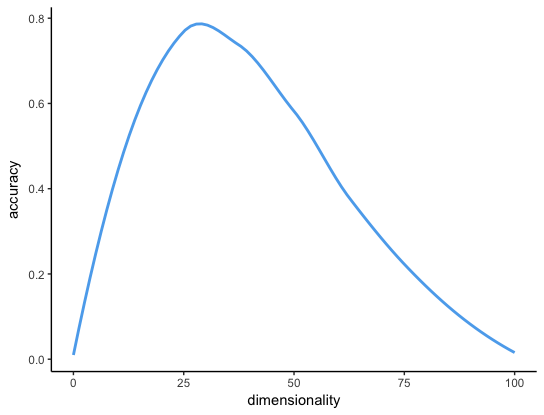
\includegraphics[width=0.8\linewidth, center]{resources/dimensionality.png}
  \caption{Hughes phenomenon}
  \label{fig:hughes}
\end{figure}

In order to reduce the dimensionality, there are two approaches can be implemented:
\begin{itemize}
  \item Feature Selection: To select a subset that is more informative or relevant among all the attributes\cite{hastie/etal:2009}.
  \item Feature Extraction: To generate new features from the initial attributes of existing data\cite{wiki/fs:2018}.
\end{itemize}

The reasons and benefits of executing dimensionality reduction can be summarised as follow:
\begin{enumerate}
  \item Computational efficiency: Fewer features mean less computation on dissimilarity between pairs of data points and lower arithmetic complexity. It also implies less storage usage as the variables in each sample decrease.
  \item Statistical generalisation: By removing noise or irrelevant information from the inputs for building models, the prediction rules can be more general among the datasets.
  \item Better explanation: Visualising a lower-dimensional space is much easier. We can effortlessly illustrate the structure of data when the dimension is lower than 3. Higher-dimensional space will be more challenging to visualise, explain and comprehend.
\end{enumerate}

Principal component analysis(PCA) is a method for feature extraction. It projects features onto a lower-dimensional space. A traditional PCA is a kind of single representation approach as opposed to classification on revealing underlying information in a lower-dimensional space with a linear function.

In practice, an optimal mapping function is usually non-linear. In order to fit the data in a non-linear way, we can apply a kernel method on top of the traditional PCA, and this is called kernel PCA. It performs a linear PCA mapping in a higher dimensional kernel Hilbert space to provide a better classification. The kernel can be a polynomial function, a radial function or other functions\cite{hessam/kpca:2014}. However, in this project, we will assume that the relationship between the dimensions (cryptocurrencies) are linear and will only use a standard linear PCA to perform the dimensionality reduction.

\subsubsection{Principal Components}

The new features derived are called principal components (PCs). They represent new orthogonal axes in an order based on the amount of information it contains.

Imagine that we have a dataset X with data points $\{{x_1} ... {x_n}\}$. Each point is a D-dimensional vector. The goal is to project the data points onto a M-dimensional space where $M < D$ and maximise the variance of data after projection. The dimensions will be the top M principal components which represent the most informative new features. M is generally determined by the following factors:

\begin{itemize}
  \item Informativity: How much information of the original features has been involved?
  \item Interpretability: Are we able to visualise or make useful attribution among the principal components?
  \item Computational efficiency: The curse of dimensionality. A large number of dimensions will decrease the speed of computation in algorithms.
\end{itemize}

% TODO equations, pseudocode, explanation chart

% \cite{bishop/praml:2006}

\subsection{Clustering}

Clustering, cluster analysis or data segmentation is a non-parametric algorithm in the subtree of unsupervised learning. It is used to separate data into different groups using their dissimilarities (similarities) or possible distributions. Unlike supervised learning, this type of learning algorithms does not have any indicator for assessing the quality of results, and this means that it does not have any meaning or objective itself. Instead, it discovers the distribution of data and uses the definition given by people who have the specific domain knowledge. By giving the rules for partitioning data self-defined meanings, useful information can be obtained and utilised in different domains\cite{hastie/etal:2009}.

In general, clustering can be defined into two types, parametric and non-parametric. A parametric clustering groups the clusters with a a assumed density function which is usually a Gaussian, while a non-parametric one does not have any assumed distribution, it only aims on finding natural groupings within the givien dataset.

K-means clustering and hierarchical clustering are two of the most popular methods in the non-parametric cluster analysis. In K-means clustering, we specify the number of groups we want to classify into. In contrast, hierarchical clustering does not have an initial number of clusters that we want for the result. It instead shows all the possible clusters into a tree structure and allows us to choose the number of clusters we want at the end. In this project, we will only focus on the K-means algorithm in non-parametric methods.

\subsubsection{K-means Clustering}

K-means clustering is a intuitive approach which allows us to separate data points into distinct groups. To implement this, we first need to specify an initial number of clusters - K, and then randomly assign a number (cluster) from 1 to K to each object (data point). In this case, the clusters will have two features\cite{james/itsl:2009}:
{
  \begin{enumerate}
    \item ${C_1}\cup{C_2}\cup...\cup{C_K} = \{{O_1}, {O_2},..., {O_n}\}$
    \item ${C_k}\cap{C_{k^\prime}} = \emptyset \text{,}\quad \text{for} \wedge k \neq k^\prime$
  \end{enumerate}

  \footnotesize
  where:
    \begin{itemize}[label=-, leftmargin=4em, itemsep=0.1em]
      \item ${C_k}$ is the kth cluster
      \item ${O_n}$ is the nth object
    \end{itemize}
}

These properties mean that each single object will be in exactly one cluster and the clusters does not overlap. After this initial setting, we want to optimise\eqref{eq:2.7} the grouping because the previous assignment is just a random initialisation. We want to make sure that the objects are concentrated which means the data point fit the best in the assigned cluster.

{
  \begin{equation}
    \label{eq:2.7}
    \tag{2.7}
    {{\underset {\mathbf {C_1,...,C_K} }{\operatorname {minimize} }}\left\{\sum _{k=1}^{K}\,{\frac {1}{|C_{k}|}}\,\sum _{ {i} , {i^\prime} \in C_{k}}\sum_{j=1}^{p}(x_{ij}-x_{{i^\prime}j})\right\}}
  \end{equation}

  \footnotesize
  where:
  \begin{itemize}[label=-, leftmargin=4em, itemsep=0.1em]
    \item ${C_k}$ is the kth cluster
    \item ${x_{ij}}$ is the jth attribute of the ith object
  \end{itemize}
}

To fulfil the condition above which is \eqref{eq:2.7}, we can simplify the apporach as below to classify our data points into the multiple clusters\cite{james/itsl:2009}:
{
  \begin{enumerate}
    \item Randomly assign an initial number from 1 to K to each observation.
    \item Iterate over the following steps until the assigned cluster of each observation stops changing:
    \begin{enumerate}
      \item for i in range(1, K): \\
      Compute the centroid of each cluster which is the mean of vectors with the same k (cluster) assigned.
      \item Calculate the distance (usually Euclidean distance) between each object and each of the clusters.
      \item  Assign the nearest k (cluster) to each observation.
    \end{enumerate}
  \end{enumerate}
}
Figure \ref{fig:kmeans} shows the difference after an optimisation of the cluster assignment. The colors indicate different clusters, and the groups are separated after the implementation of K-means clustering.

\begin{figure}[ht]
  \centering
  \figuretitle{K = 4}
  \begin{subfigure}[b]{0.48\textwidth}
    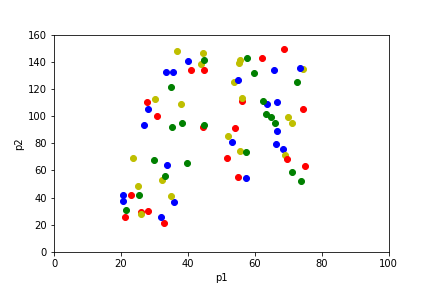
\includegraphics[width=\linewidth, center]{resources/kmeans_before.png}
    \caption{Before Iteration}
    \label{fig:before_iter}
  \end{subfigure}
  \begin{subfigure}[b]{0.48\textwidth}
    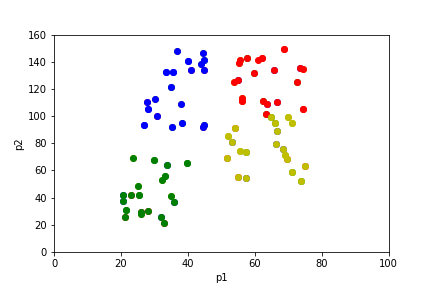
\includegraphics[width=\linewidth, center]{resources/kmeans_after.png}
    \caption{After Iteration}
    \label{fig:after_iter}
  \end{subfigure}
  \caption{K-means Clustering}
  \label{fig:kmeans}
\end{figure}

\subsubsection{Dynamic Time Warping Distance}

Euclidean distance is a metric for evaluating the distance between sequences. It is useful as it produces non-negative result and has linear time complexity. However, it is restricted by the alignment of sequences, which means that the distance can only be calculated if the two sequences are in the same length. If we want to learn how similar the shapes of two objects/lines in time series are, this is not a good method to be used.

Dynamic time warping (DTW) is a popular shape-based algorithm based on dynamic programming in time series analysis. DTW is a time distortion method which adjusts the corresponding elements in two vectors and finds the minimal distance among the neighbours. The accumulative value will then become the final distance in between. It is widely used in temporal sequence data such as speech recognition\cite{aggarwal/data:2013}.

Given two vectors $t$ and $r$, and the lengths are $M$ and $N$ respectively, DTW aims on finding a path to minimise the distance between $t$ and $r$.

\begin{figure}[ht]
    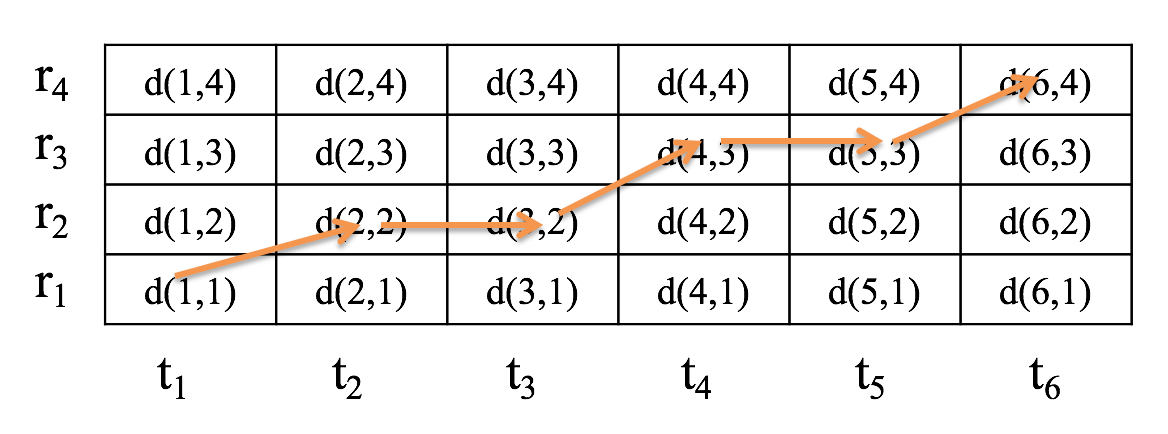
\includegraphics[width=0.8\linewidth, center]{resources/DTW_path.png}
    \caption{DTW Optimal Path}
    \label{fig:dtwpath}
\end{figure}

The calculation of the DTW distance needs to satisfy the following conditions\cite{wiki/dtw:2018}:
{
  \begin{enumerate}
    \item The first element from $t$ must match the first element from $r$.
    \item The last element from $t$ must match the last element from $r$.
    \item Given $d(i,j)$ is the distance of a point on the optimal path. The points that connect into $d(i,j)$ can only be $d(i-1,j)$, $d(i-1,j-1)$ and $d(i,j-1)$.
    \item Given any element in $t$, there must be at least one corresponding element in $r$, and vice versa.
  \end{enumerate}
}

We can use a recursion\eqref{eq:2.8} to find out the minimal accumulative distance $A(M,N)$ which is our goal of the DTW distance\cite{wiki/dtw:2018}.

{
    \begin{equation}
        \label{eq:2.8}
        \tag{2.8}
        {A(i,j) = d(i,j) + min
        \left \{
            \begin{tabular}{c}
                A(i-1,j) \\
                A(i-1,j-1) \\
                A(i,j-1)
            \end{tabular}
        \right \}}
    \end{equation}

    \footnotesize
    where:
    \begin{itemize}[label=-, leftmargin=4em, itemsep=0.1em]
        \item $D(i,j)$ is the distance between $t_i$ and $r_j$
        \item $A(i,j)$ is the accumulative distance from the starting point to $(i,j)$
    \end{itemize}
}

\section{Analysis of Cryptocurrencies}

The data of cryptocurrencies is obtained from a RESTful API \url{https://min-api.cryptocompare.com/} which is free for non-profit purposes. We store the data into our local Docker based PostgreSQL database for development and convenience in case the internet or the API are unstable. Our Java programme will then update the latest data on a daily basis.

This analysis will use the historical daily OHLCV (Open price, High price, Low price, Close price, Volume) data of cryptocurrencies as the initial input obtained from the API and will only consider 29 cryptocurrencies that have complete data from \date{1st January 2016} to \date{31st July 2018}. The reason why we choose the number 29 is because we want to compare the performance on cryptocurrencies with that on stocks and we will choose Dow Jones 30 as our counterpart. We want to make them have the same size of products and DWDP in Dow Jones does not have the data before \date{1st September 2017}.

\subsection{Data Preprocessing}

The original data of cryptocurrencies contains the open price, highest price, lowest price, close price and volume changes of different cryptocurrencies for each day. The unit of the price is USD. There is no specific trading hours for cryptocurrencies. The metric the API used to split the values into days is based on 00:00 GMT time. For simplicity, we will use symbols to represent cryptocurrencies. Table \ref{table:symbolcrypto} shows the corresponding cryptocurrency of each symbol.

{
  \begin{table}[ht]
    \centering
    \small
    \begin{tabular}{|c|c|c|c|c|c|}
        \hline
        Symbol & Crypto & Symbol & Crypto & Symbol & Crypto \\
        \hline
        AEON & Aeon & BAY & BitBay & BLOCK & Blocknet \\
        BTC & Bitcoin & BTCD & BitcoinDark & BURST & Burst \\
        CRW & Crown & DASH & Dash & DGB & DigiByte \\
        DOGE & Dogecoin & EMC2 & Einsteinium & ETH & Ethereum \\
        FCT & Factom & FTC & Feathercoin & GAME & GameCredits \\
        GRS & Groestlcoin & LTC & Litecoin & MONA & MonaCoin \\
        NAV & NavCoin & NLG & Gulden & POT & PotCoin \\
        PPC & Peercoin & RDD & ReddCoin & SYS & Syscoin \\
        VIA & Viacoin & VTC & Vertcoin & XCP & Counterparty \\
        XMR & Monero & XRP & Ripple & & \\
        \hline
    \end{tabular}
    \caption{Symbols of Cryptocurrencies}
    \label{table:symbolcrypto}
  \end{table}
}

Before we start our analysis, we need to preprocess the data to ensure that the data is clean enough and in the format which can be used as the input of the analysis. The historical daily OHLCV data requested from the API is on the crypto by crypto basis. In this case, we extract all the data, combine them into the format of Table \ref{table:ohlcvcrypto} and store them into the database.

{
  \begin{table}[ht]
    \centering
    \scriptsize
    \begin{tabular}{|c|c c c c c c|}
      \hline
       & AEON\_open & AEON\_high & AEON\_low & ... & XRP\_close & XRP\_volume \\ [0.5ex]
      \hline
      2016-01-01 & 0.01454 & 0.0217 & 0.01316 & ... & 0.0055 & 0 \\
      \hline
      2016-01-02 & 0.01498 & 0.01734 & 0.01388 & ... & 0.005125 & -496.94 \\
      \hline
      2016-01-03 & 0.01378 & 0.01536 & 0.01379 & ... & 0.0052 & -23.8623 \\
      \hline
      2016-01-04 & 0.01391 & 0.0143 & 0.01218 & ... & 0.0051 & 0 \\
      \hline
      ... & ... & ... & ... & ... & ... & ... \\
      \hline
      2018-07-28 & 1.58 & 1.75 & 1.58 & ... & 0.4576 & -6853079.88 \\
      \hline
      2018-07-29 & 1.67 & 1.78 & 1.58 & ... & 0.4529 & -5774418.55 \\
      \hline
      2018-07-30 & 1.68 & 1.69 & 1.57 & ... & 0.4458 & -15453544.47 \\
      \hline
      2018-07-31 & 1.55 & 1.55 & 1.42 & ... & 0.4351 & -16047905.37 \\
      \hline
    \end{tabular}
    \caption{Historical OHLCV of Cryptocurrencies}
    \label{table:ohlcvcrypto}
  \end{table}
}

Our objective is to evaluate the risk based on price volatility which is the daily price changes ($g$) or daily rate of return ($r$). We can calculate the daily price changes through dividing the close price by the open price. The rate of return ($r$) is then equal to $1 - g$. Table \ref{table:dccrypto} shows the daily price changes after transformation from the historical OHLCV dataset.

{
  \begin{table}[ht]
    \centering
    \scriptsize
    \begin{tabular}{|c|c c c c c c c|}
      \hline
       & AEON & BAY & BLOCK & ... & XCP & XMR & XRP \\ [0.5ex]
      \hline
      2016-01-01 & 0.030949 & -0.296502 & -0.265306 & ... & -0.038405 & 0.108141 & 0.056676 \\
      \hline
      2016-01-02 & -0.073431 & 0 & 0.180451 & ... & -0.033988 & -0.153010 & 	-0.001364 \\
      \hline
      2016-01-03 & 0.002903 & -0.085601 & -0.036252 & ... & -0.025285 & 0.059783 & 0.014634 \\
      \hline
      2016-01-04 & -0.097052 & 0.124730 & 0.009491 & ... & 0.048847 & -0.035897 & -0.019231 \\
      \hline
      ... & ... & ... & ... & ... & ... & ... & ... \\
      \hline
      2018-07-28 & 0.056962 & -0.024547 & 0.012285 & ... & -0.005362 & -0.000714 & 0.006157 \\
      \hline
      2018-07-29 & 0.011976 & 0.002037 & -0.040519 & ... & -0.028340 & -0.030859 & -0.010487 \\
      \hline
      2018-07-30 & -0.023810 & -0.016599 & -0.078947 & ... & 0 & -0.025429 & -0.015677 \\
      \hline
      2018-07-31 & -0.064516 & -0.059292 & -0.094542 & ... & -0.098820 & -0.076615 & -0.024002 \\
      \hline
    \end{tabular}
    \caption{Historical Daily Changes of Cryptocurrencies}
    \label{table:dccrypto}
  \end{table}
}

\subsection{Risk Estimation}
\subsubsection{Historical Estimation of VaR}
\subsection{Risk Diversification}
\subsubsection{Product Correlations}
\subsubsection{Clustering on Price Movement}
\subsection{Performance}
\subsubsection{Back Test}
\subsubsection{Improvement After Risk Diversification}

\section{Analysis of Stocks}
\subsection{Data Preprocessing}
\subsection{Risk Estimation}
\subsubsection{Historical Estimation of VaR}
\subsection{Risk Diversification}
\subsubsection{Product Correlations}
\subsubsection{Clustering on Price Movement}
\subsection{Performance}
\subsubsection{Back Test}
\subsubsection{Improvement After Risk Diversification}

\clearpage

\section{Evaluation and Conclusion}
\subsection{Comparison Between Cryptocurrencis and Stocks}
\subsection{Trading Strategy}
\subsection{Further Work}

\section{Appendix}
\subsection{Programme Usage}

\bibliographystyle{plain}
\bibliography{bibliography}
\end{document}
